%!TEX root = ../dissertation.tex

\chapter{Results Discussion}

\newthought{The methods} described in Chapter 3 were implemented and tested for their efficacy at evaluating average causal treatment effect.  Results and discussion are presented here.  

\section{Natural Course} 
In order to test the specified models used for the g-formula method, a natural course study was performed.  This involved simulating the data directly using the models specified for the g-formula method.  Additionally, a model for the treatment variable had to be created as well, giving the following three models,\footnote{Abbreviated models, like those specified in expressions \ref{eq:6} and \ref{eq:7}, were used for time points $t=0,1,2$ since adequate historical data is not available.} 
\begin{align} 
Logit \big[Y \mid \overline{A}_t, \overline{L}_t \big] &= \theta_{0} + \theta_1 A_{t} + \cdots + \theta_j A_0 + \theta_{j+1} L_t + \cdots + \theta_{j+k} L_0  \\ 
logit[L_k \mid \overline{L}_{k-1}, \overline{A}_{k-1}] &= \gamma_0 + \gamma_1 L_{k-1} + \gamma_2 L_{k-2} + \gamma_3 L_{k-3}  + \gamma_4 A_{k-1} + \gamma_5 A_{k-2} + \gamma_6 A_{k-3} \\ 
logit[A_k \mid \overline{L}_{k}, \overline{A}_{k-1}] &= \delta_0 + \delta_1 L_{k} + \delta_2 L_{k-1} + \delta_3 A_{k-1} + \delta_4 A_{k-2} 
\end{align} 

Five new data sets were simulated to determine the natural course of these models.  Table \ref{naturalcourse} below compares the true mean of the original data frame and the average across the five simulated dataframes.  


\begin{table}[h!]
\centering
\begin{tabular}{c | c c c}
Variable & True Mean & \shortstack{Natural Course\\ Average Mean} & \shortstack{Natural Course \\95\% CI} \\ 
\hline \\
$\mathbb{E}[Y]$ & 0.714 & 0.719 & (0.705, 0.733) \\ \\
$\mathbb{E}[A]$ & 0.848 & 0.847 & (0.840, 0.854) \\ \\
$\mathbb{E}[L]$ & 0.833 & 0.811 & (0.793, 0.830) 
\end{tabular} \\
\centering
\caption{A table outlining the results of the natural course test of the methods.  True mean is specified using the underlying dataset which the models are created off of.  The natural course average mean is the mean of means from the five datasets.  The 95\% confidence interval is centered at this mean of means and based on the five datasets. \label{naturalcourse}}
\end{table}

The results of the natural course in Table \ref{naturalcourse} show that the models chosen appear to estimate the data quite well.  Not only are the means close to the true mean, but the variance is low enough that our confidence intervals all cover the true mean.  Therefore, it can be concluded that these models are a good choice for adequately modeling the underlying data in the g-formula.  

\section{Simulation of the Two Methods} 
As discussed in Section \ref{VarianceBootStrap}, a simulation of 1,000 iterations was performed.  Each iteration of this simulation consisted of creating a new dataset and obtaining both the g-formula estimate and the doubly robust estimate for the causal treatment effect.  

The results of these simulations can be seen below in Table \ref{simdata} and Figure \ref{bighistogram}.  Both indicate that the doubly robust method has a more precise average causal treatment effect across simulations.\footnote{As discussed in Section \ref{data}, no effect of $A$ on $Y$ was included in this study, so the true causal treatment effect should be zero.}  However, this improvement comes with higher variance and bias, as shown in the wider confidence interval and the larger spread on the histogram.  

Furthermore, the relationship between the data and the causal effect estimates was examined in Figure \ref{correlation}.  Of note, the doubly robust method is able to capture correlation between $Y$ and $A$ which the g-formula method does not, an important indicator that it successfully picks up treatment effect.  This likely contributes to the more precise causal treatment effect measure.  

\begin{table}[h!]
\centering
\begin{tabular}{c | c c c c }
Method & \shortstack{Average Causal \\ Treatment Effect} & Average Bias & \shortstack{Variance of \\ Effect Estimate} & \shortstack{95\% Conf. Int.\\ of Effect Estimate} \\ 
\hline \\
G-Formula & 0.0033 & 0.016 & 0.00024&(-0.00063,0.00128)\\ \\ 
Doubly Robust & 0.00026 & 0.031& 0.00079 & (-0.00149, 0.00212)
\end{tabular} \\
\centering
\caption{A table presenting the results of 1,000 data simulations, within which the g-formula and doubly robust estimators of average causal effect were each obtained.  Average causal treatment effect is the mean of the causal treatment effect across the simulations.  The variance and confidence intervals reflect the variability in that causal treatment effect over 1,000 simulations. \label{simdata}}
\end{table}

\begin{figure}[h!]
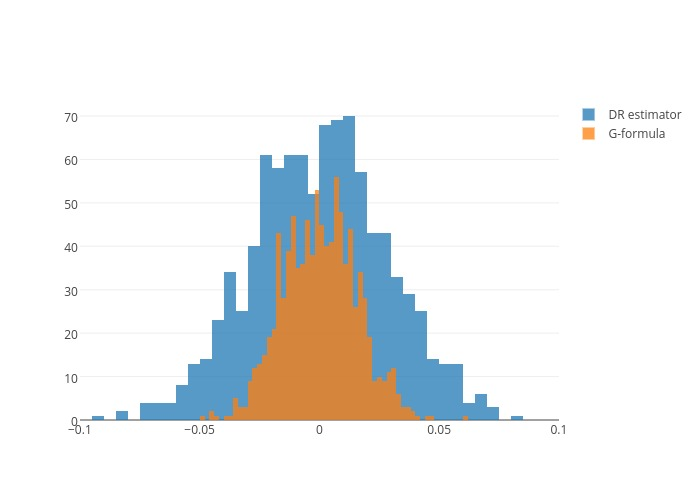
\includegraphics[width = \linewidth]{figures/overlaid_histogram.jpeg}
\caption{A histogram showing the results of the 1,000 simulations.  The y-axis shows frequency of value and the x-axis shows the causal treatment effect value measured.}
\label{bighistogram}
\end{figure} 

\begin{figure}[h!]
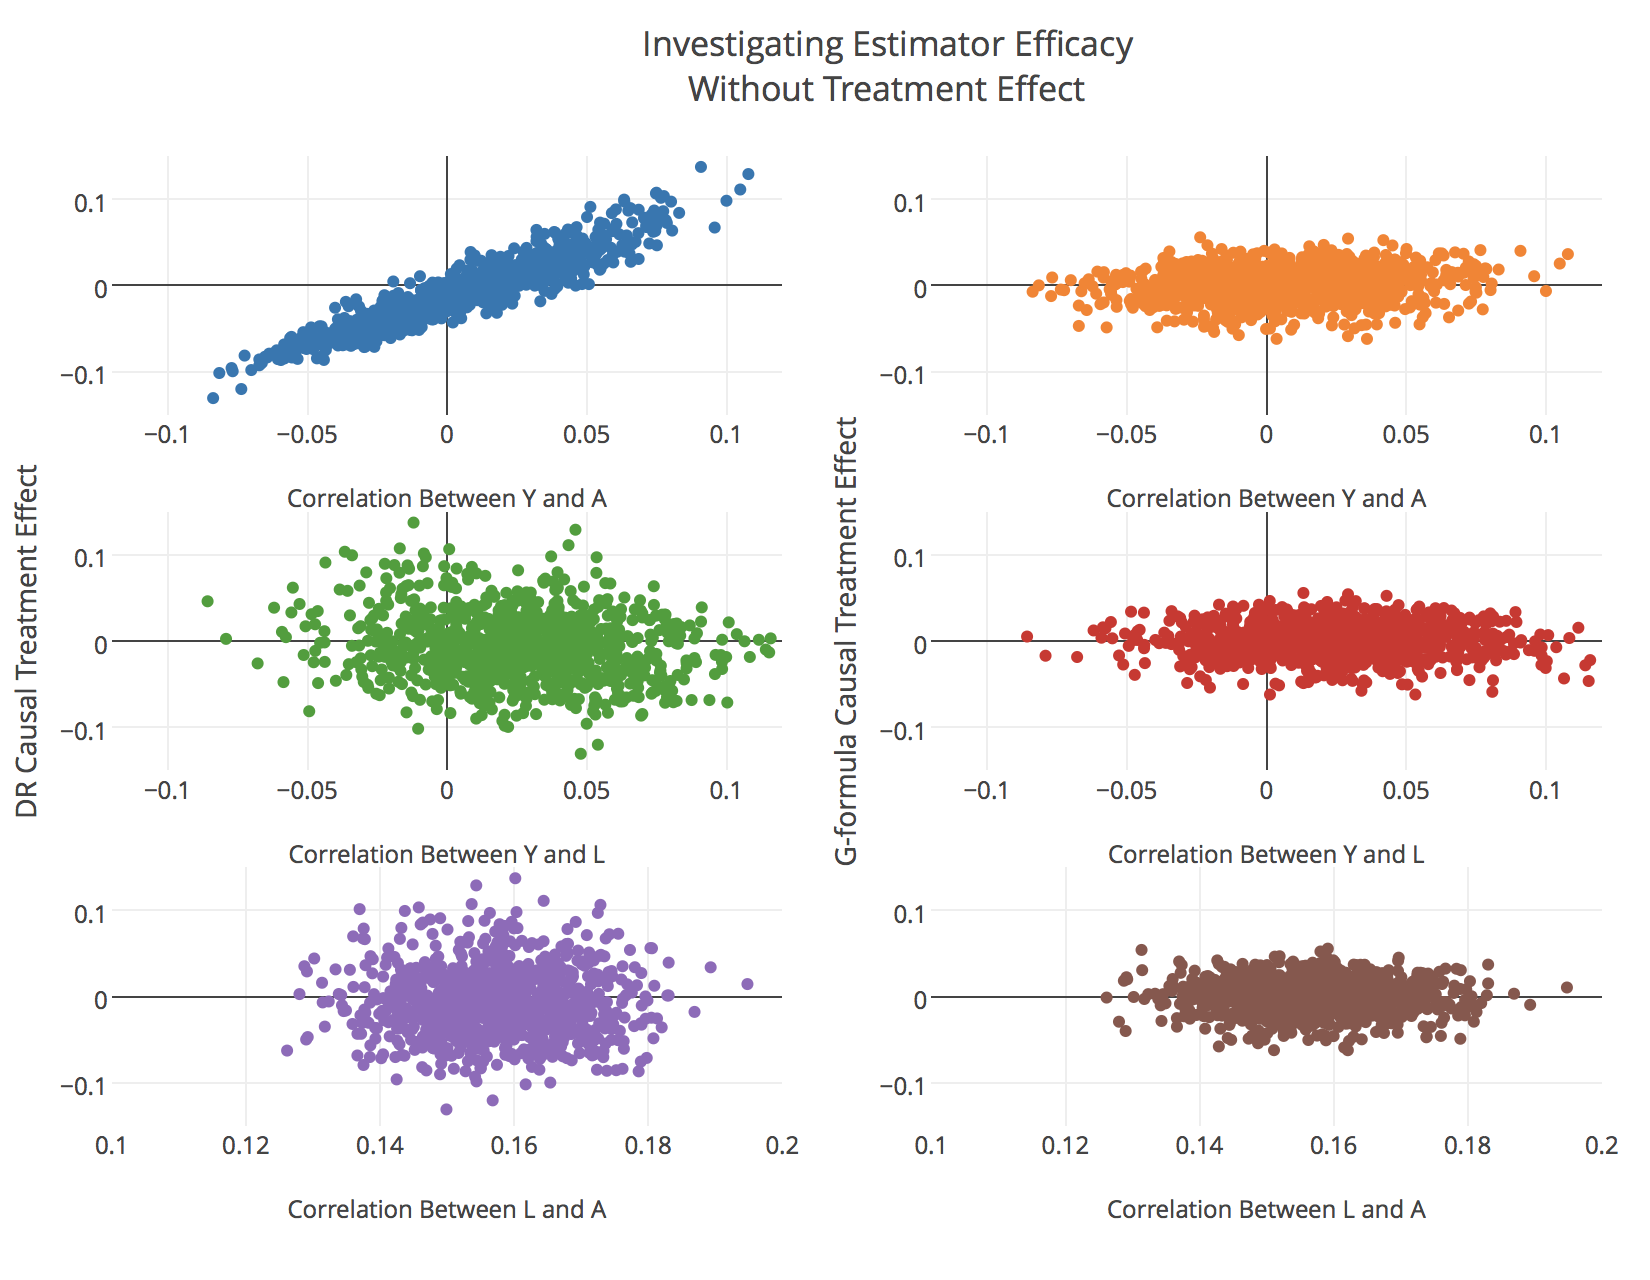
\includegraphics[width = 1.1\linewidth]{figures/correlation.png}
\caption{Various plots showing the relationship between underlying data correlations and estimated causal treatment effects using the two methods.  Each data point is representative of one dataset.  The same 1,000 datasets are used for each effect estimation.}
\label{correlation}
\end{figure}

\newpage
\section{Confirming Double Robustness} 
Twenty-five simulations were performed in order to test the double robustness of the ``doubly'' robust estimator.  Four different setups were tested: 
\begin{itemize} 
\item Using the correctly specified model for both user specified functions, $\hat{\mathbf{\alpha}}$ and $s_{m-1}$ 
\item Using an intentionally misspecified model for $\hat{\mathbf{\alpha}}$ while keeping the correct model for $s_{m-1}$ 
\item Using an intentionally misspecified model for $s_{m-1}$ while keeping the correct model for $\hat{\mathbf{\alpha}}$
\item Using intentionally misspecified models for both $\hat{\mathbf{\alpha}}$ and $s_{m-1}$ 
\end{itemize} 

The misspecified models used were as follows, 
\begin{align} 
f(A_m \mid \overline{L}_m, \overline{A}_{m-1}; \hat{\mathbf{\alpha}}) &= \alpha'_{0} + \alpha'_{1} \cdot L_{m-3} + \alpha'_{2} \cdot A_{m-3} \\ 
s_{m}(\overline{L}_{m}, \overline{A}_{m};\mathbf{\beta}_{m}) &= \theta'_0 + \theta'_1 A_{m} +\theta'_2 L_m  +\theta'_3 A_{m-4} +  \theta'_4 L_{m-4} 
 \end{align} 
These models were chosen because they are quite random, and it would be unlikely based on the knowledge of how the data was created that these would be strong models for prediction.  In practice, one would hope that the researcher using these methods would be wiser as not to use such terrible models, particularly for both models.  

The results of this testing are shown in Table \ref{doubletest} and this shows evidence that the method is indeed doubly robust.  This means that when one model is incorrect, but the other is correct, then the estimate should not be biased.  The average causal treatment effect across the simulations is not significantly impacted when either the $\hat{\mathbf{\alpha}}$ model or the $s_{m-1}$ model is incorrectly specified.  When both models are misspecified, statistically significant bias is introduced (p-value 0.005).  Furthermore, both Table \ref{doubletest} and Figure \ref{boxplot} show that the variance is significantly higher when both models are misspecified.  From the boxplot, it can be seen that the variance stays quite consistent when only one model is misspecified but is much larger when both are misspecified.  


\begin{table}[h!]
\centering
\begin{tabular} {c | c  c c}
Models & \shortstack{Average Bias in Causal \\ Treatment Effect} & p-value & \shortstack{Standard Error\\ of Bias} \\ 
\hline  \\
Both models correctly specified &0.027 & NA  & 0.0039\\ \\
$\hat{\mathbf{\alpha}}$ correct, $s_{m-1}$ misspecified & 0.030 & 0.579 & 0.0041\\ \\
$\hat{\mathbf{\alpha}}$ misspecified, $s_{m-1}$ correct & 0.030 & 0.521 &0.0042 \\ \\
Both models misspecified & 0.133 & 0.005 & 0.0355 
\end{tabular} \\
\centering
\caption{Table showing the results of testing the double robustness of the model.  The p-value is from a two-sample t-test comparing the bias from misspecified versions with the bias results from having both models correctly specified. \label{doubletest}}
\end{table}

\begin{figure}[h!] 
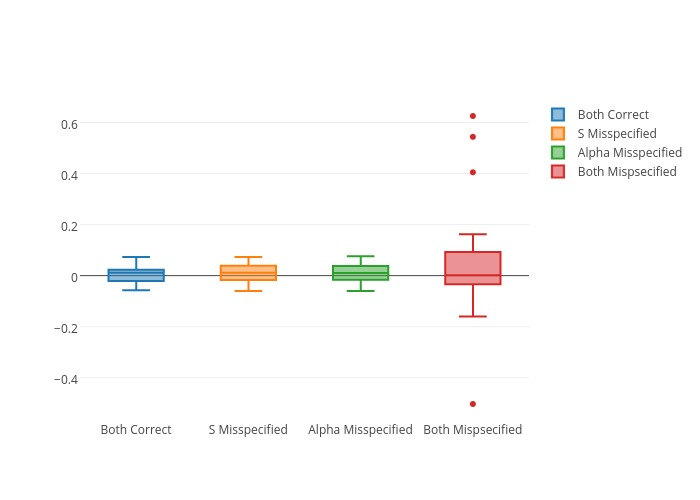
\includegraphics[width = \linewidth]{figures/boxplot.jpg}
\caption{}
\label{boxplot}
\end{figure} 



\newpage
\section{Testing Multiple Robustness} 

\begin{table}[h!]
\centering
\begin{tabular} {c | c  c}
Model Correctly Specified & \shortstack{Average Bias \\ of Estimate}  & \shortstack{Variance \\of Estimate} \\ 
\hline  \\
$\pi_3, \dots, \pi_K$ & 0.026 & 0.0013   \\ 
$\pi_3, \dots, \pi_{K-1}, s_K$ & 0.024 & 0.0010\\ 
$\pi_3, \dots, \pi_{K-2}, s_{K-1}, s_K$ & 0.023 & 0.0010\\ 
$\pi_3, \dots, \pi_{K-3}, s_{K-2} , s_{K-1}, s_K$ & 0.023  &0.0009 \\ 
$\pi_3, \dots, \pi_{K-4}, s_{K-3}, \dots s_K $ & 0.023&0.0009 \\ 
$\pi_3, \dots, \pi_{K-5}, s_{K-4}, \dots s_K $ &  0.023 &0.0009\\ 
$\pi_3, \dots, \pi_{K-6}, s_{K-5}, \dots s_K $ &  0.023 & 0.0009 \\ 
$\pi_3, \dots, \pi_{K-7}, s_{K-6}, \dots s_K $ &  0.024 & 0.0010\\ 
$\pi_3, s_{4}, \dots s_K $ &  0.025& 0.0011  \\ 
$s_3, \pi_4, \dots \pi_K$ &  0.196 & 0.0881 \\ 
$s_3, s_4, \pi_5, \dots \pi_K$ & 0.08 & 0.0214  \\ 
$s_3, s_4, s_5, \pi_6, \dots \pi_K$ & 0.052 & 0.0100  \\ 
$s_3, \dots s_6, \pi_7, \dots \pi_K$ & 0.064 &0.0206 \\ 
$s_3, \dots s_7, \pi_8, \dots \pi_K$ &  0.060 &  0.0195   \\ 
$s_3, \dots s_8, \pi_9, \dots \pi_K$ & 0.048 &0.0129   \\ 
$s_3, \dots s_9, \pi_{10}, \pi_K$ &  0.028 & 0.0015 \\ 
$s_3, \dots s_{10}, \pi_K$ & 0.027 & 0.0013 \\
$s_3, \dots s_K$ & 0.026 & 0.0013\\ 
\end{tabular} \\
\centering
\caption{Hi?}
\end{table}

\begin{figure}
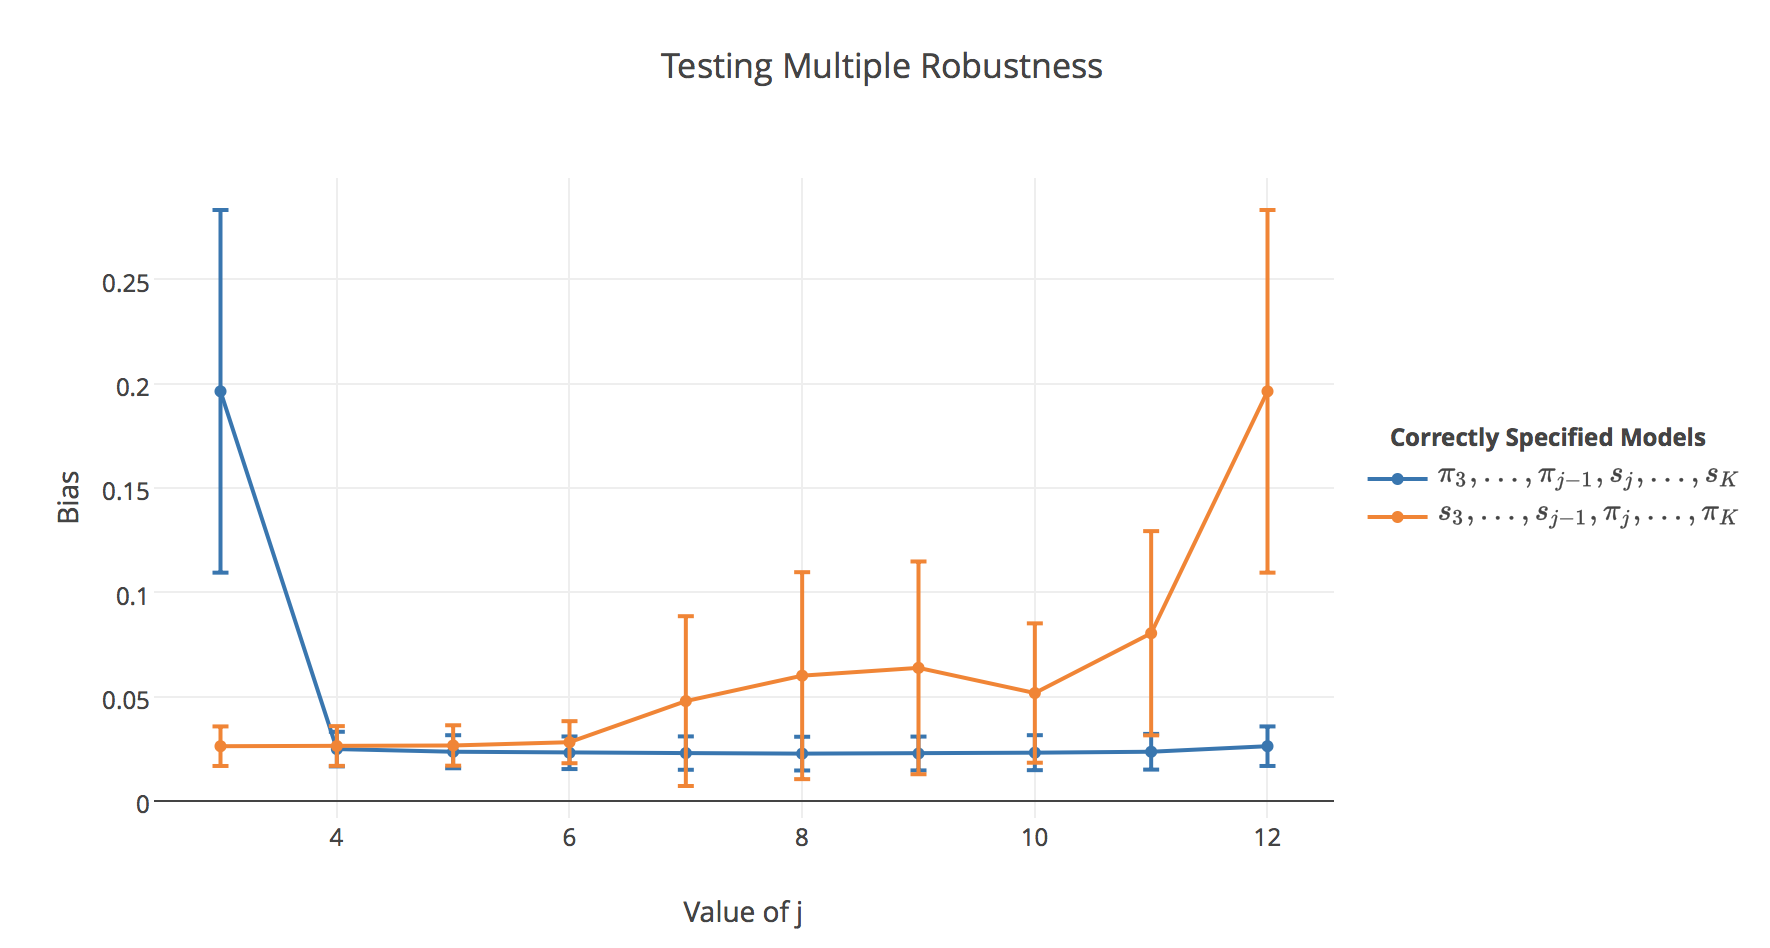
\includegraphics[width = 1.1\linewidth]{figures/multiplerobust.png}
\caption{}
\label{multirobust}
\end{figure} 

\begin{figure}
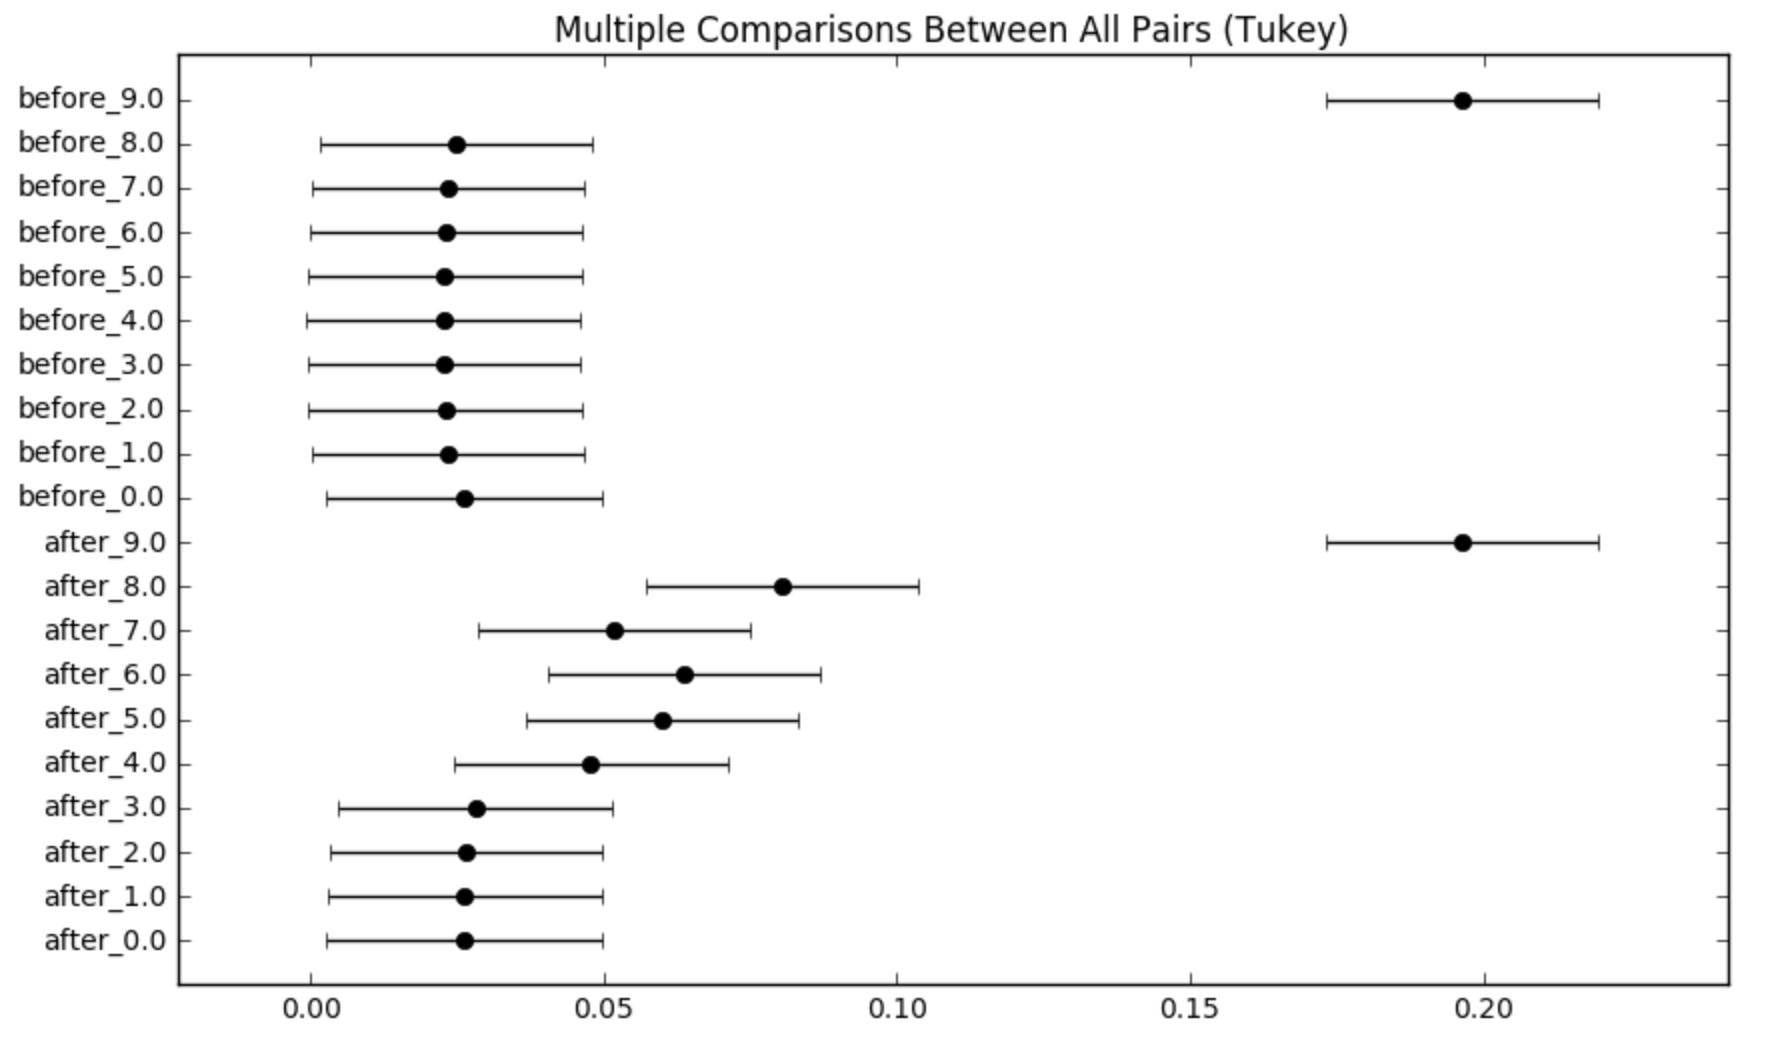
\includegraphics[width = 1.1\linewidth]{figures/Tukey.png}
\caption{A plot of the confidence intervals of each of the model specifications in the testing of multiple robustness.  The y-axis indicates which model, where the number is the value of $j$ in the following models, the before model is $\pi_3,\dots, \pi_{j-1},s_j,...,s_K$ and the after model is $s_3, \dots, s_{j-1}, \pi_j, \dots, \pi_K$.  The before and after notation signifies whether the $\pi$ models are correctly specified in order before or after the $s_m$ models.  The before values correspond to the blue lines in Figure \ref{multirobust} while the after values correspond to the orange line.}
\label{Tukey}
\end{figure} 


